\documentclass{article}

\usepackage{color}
\usepackage{fullpage}
\usepackage{graphicx}
\usepackage{multicol}
\usepackage{multirow}
\usepackage{outline}
\usepackage{url}

\newcommand{\FIXME}[1]{\textcolor{blue}{[\textbf{FIXME}: {#1}]}}

\twocolumn


\title{Tweedr: Twitter for Disaster Response}
\author{Zahra Ashktorab \and Chris Brown \and Jit Nandi \and Aron Culotta}


\begin{document}
\maketitle

\section{Introduction}

\begin{outline}
  \item Context
  \item Problem
  \item Solution Overview
\end{outline}
In recent years, Twitter has become a major channel for communication during natural disasters. From \#snowpocalypse to \#Sandy, Twitter users have shared news, photos and observations from the midst of hurricanes, blizzards, earthquakes and other emergencies. First responders can utilize these streams of data generated by social media to find out where the disasters are happening and what specifically has been effected as a result of it.
As with most social media conversations, informative signals are often drowned out by irrelevant and redundant noise. First responders struggle to glean actionable knowledge from the flood of tweets and status updates.
In order to solve this problem, we propose the Tweedr: a tool that extracts relevant information to first responders from tweets generated during disasters. The tweedr pipeline consists of three main parts: classification, clustering and extraction. In the classification phase, we use a variety of classification methods (sLDA, SVM, and LogReg) to classify whether a tweet reports disaster damage information. In the clustering phase, we merge utilize filters to merge tweets that are similar to one another, and finally in the extraction phase, we extract specific tokens and phrases that report specific information about different classes of infrastructure damage and damage types. Using these three phases, the Tweedr pipeline is able to extract actionable information from a stream of tweets during disasters.

\section{Data}
\begin{outline}
  \item Unlabeled data from different disasters
  \item Labeling for classification (and uniform vs keyword sampling)
  \item Labeling for extraction
  \item Summary statistics (number labeled/unlabeled; number of each class; number by disaster)
\end{outline}

We identified 12 crisis events that occurred in North America since the
founding of Twitter in 2006. We then constructed queries to collect relevant
tweets from Gnip, a social media aggregation company. We constructed two types
of queries: (1) keyword ({\bf kw}) queries contain search terms and hashtags
determined to be relevant based on a post-hoc analysis; (2) geographical
queries ({\bf geo}) consisting of a bounding box of coordinates around the
epicenter of the event. Table \ref{tab.data_summary} lists the number of
tweets collected for each event.

In a real-world deployment, it may be difficult to manually construct a list
of keywords relevant to a disaster, but we leave this for future work.

\begin{table*}
\centering
\small
\begin{tabular}{|l|r|r|r| p{8cm} |}
\hline
{\bf Event}  & {\bf N (kw)} & {\bf N (geo)} & {\bf total} & {\bf keywords} \\
\hline
christchurch &  759,399  & 2,017       &  761,416    & \#EQNZ,\#CHCH,\#NZquake,Christchurch\\
ike          &  113,773  & 3,989       &  117,762    & Hurricane+Ike,Hurricane,Ike,Galveston,Houston\\
irene        &  384,689  & 3,871,631   &  4,256,320  & \#Hurricane,\#Irene,\#Tropics\\
moore        &  842,318  & 1,579,056   &  2,421,374  & \#mooretornado,\#moore,newcastle\\
oklahoma     & 1,697,891 & 6,209,510   &  7,907,401  & \#oklahoma,\#tornado,\#oklahomatornado,\#okwx,\#okc\\
samoa        & 235,208   &  2,016      &  237,224    &  Samoa,tsunami,earthquake\\
slavelake    & 45,072    &  1,281      &  46.353     & \#SlaveLake,Slave+Lake\\
supertuesday & 22,205    &  2,201      &  24,406     & Super+Tuesday,Jackson,Memphis,supertuesday\\
tornado2011a & 476,730   &  2,293      &  479,023    & Tushka,oklahoma,okwx,arkansas,akwx,tornado\\
tornado2011b & 52,201    &  2,326      &  54,527     & \#alwx,\#okwx,\#txwx,\#tristatewx,tornado,\mbox{\#ALNeeds}, \#ALHaves,\#WeAreAlabama\\
vtech        & 16,652    &  2,869      &  19,521     & \#vatech,\#virginiatech,\#hokies,\#vtech,\#vt\\
westtx       & 651,045   &  178,846    &  829,891    & \#WestExplosion,\#WestTX\\
\hline
{\bf Total}  & {\bf 5,297,183} & {\bf 11,858,035}  & {\bf 17,155,218}  &\\
\hline
\end{tabular}
\caption{Number of tweets collected by event. We query for tweets both by
  keyword ({\bf kw}) and geographical bounding box ({\bf geo}).\FIXME{Sort by
    year or size?}\label{tab.data_summary}}
% See dssg-twitter-disaster/aron/count_lines.py
\end{table*}

\subsection{Data Annotation}
To train and evaluate our automated methods, we must first collect
human-annotated examples. We consider two tasks for annotation:
\begin{enumerate}
  \item {\bf Classification}: Does the tweet mention either specific
    infrastructure damage or human casualty? We treat this as a binary
    classification task. Positive examples include ``10 injured in plant
    explosion'' and ``The windows are smashed at the Whole Foods on 1st'';
    however, ``Hurricane Irene causes massive damage'' would be a negative
    example, since it does not include specific, actionable damage
    information.
  \item {\bf Extraction}: For positive examples of the above, identify the
    tokens in the tweet corresponding to specific types of infrastructure
    damage or counts of the number of dead or injured. For example, in the
    tweet ``Flooding bad up and down sides of Green River Rd,'' the token
    ``Flooding'' should be annotated as a damage type, and the tokens ``Green
    River Rd'' should be labeled as a road. The full ontology is listed in
    Table \FIXME{add}.
\end{enumerate}

Since not all data can be labeled manually, we sample a small subset. Half of
the tweets are selected uniformly at random from each event; the remaining
half are sampled from tweets matching a set of keywords heuristically
determined to be relevant to our task.\footnote{The keywords are: bridge,
  intersection, car, bus, truck, vehicle, evacuation, evacuate, fire, police,
  institution, wind, impact, injured, damage, road, airplane, hospital,
  school, home, building, flood, collapse, death, casualty, missing.} We do
this to mitigate the class imbalance problem (i.e., most tweets are not
relevant to infrastructure damage or casualties).

We sampled 1,049 tweets of the resulting tweets, of which 793 were labeled as
positive examples. We then annotate the extraction labels for each positive
example.
% mysql> select count(*) from DamageClassification where mturk_code='QCRI';
% 1049
% mysql> select count(*) from DamageClassification where mturk_code='QCRI' and Infrastructure=1 or Casualty=1;
% 793


\subsection{Classification}
We compare a number of standard classification algorithms, including
$K$-nearest neighbors, decision trees, na\"ive Bayes, and logistic regression,
as implemented in the {\tt scikit-learn} Python
library.\footnote{\url{http://http://scikit-learn.org/}} We also compare with
supervised latent Dirichlet allocation~\cite{blei10supervised}, for which we create a Python wrapper of the R {\tt lda} package.\footnote{\url{http://cran.r-project.org/web/packages/lda/}}

\subsection{Clustering}
We consider two different methods of approximate string matching: Bloom
filters~\cite{bloom70space} and SimHash~\cite{charikar02similarity}.


\subsection{Extraction}
For extraction, we use a conditional random field (CRF)~\cite{sutton12intro}, as
implemented by the {\tt CRFsuite}
toolkit.\footnote{\url{http://www.chokkan.org/software/crfsuite/}}. We consider several different types of features for our CRF. For each token in a tweet, we inspect capitalization, pluralization, whether it is numeric or includers a number, whether it is part of a determined lexicon of transportation types or building types, hypernyms, ngrams, and part of speech tags. 
To obtain precision, recall, and f1-score values, we split the data using two methods. In Table \ref{tab.by_label}, we use k-folds cross validation, where k is 10. Additionally, we split the data by disaster, training on the labeled data from our top 5 disaster and testing on the sixth. The disasters we trained on this second method include: Joplin, Irene, Samoa, Christchurch, Tornado2011b, and Oklahoma. By splitting the training and testing data on disaster, we can test the accuracy of our classifier on unseen disasters. In Table \ref{tab.unseen_disaster}, we show the overall average for the CRF for performing on an unseen disaster.
As seen by Table \ref{tab.by_label}, our entity extraction classifier performs well (obtains an f1-score above .5) on predicting missing persons, religious institutions, electricity loss, hospital and health infrastructures, death/casualties, and wind/projectile damage. However, it does not predict fires and homes/residential infrastructures as accurately as the aforementioned labels. Furthermore, due to the nature of content in tweets, there is not enough sufficient labelled data for certain labels and thus precision, recall and f1-scores could not be obtained.
We also evaluated our CRF across disasters to evaluate how it performed on disasters it had not seen yet. The results were promising for some disasters, yielding promising f1-score values for four of the six disasters evaluated. The results are reflected in Table \ref{tab.unseen_disaster}.


\section{Experiments}
\begin{outline}
  \item Classification results
    \begin{outline}
      \item overall precision, recall, f1
      \item compared with predicting on unseen disasters
      \item comparison of sLDA and vanilla classifiers
      \item visualize important features (e.g., sLDA graph)
      \item list some exemplary good/bad classifications
    \end{outline}
  \item Clustering results (maybe don't need accuracy, but at least what percent is duplicate)
  \item Extraction
    \begin{outline}
      \item overall precision, recall, f1, confusion matrix
      \item compared with predicting on unseen disasters
      \item visualize important features
      \item list some exemplary good/bad classifications
    \end{outline}
\end{outline}

\begin{table*}[t]
\centering
\begin{tabular}{|c|c|c|c|c|c|c|}
\hline
              & \multicolumn{3}{c|}{All} &                       \multicolumn{3}{c|}{New Disaster}  \\
\hline
{\bf Method}  &  {\bf F1}        &  {\bf Pr}  &  {\bf Re} & {\bf F1}  &  {\bf Pre}  &  {\bf Re}\\
\hline
{\bf sLDA}    &  0.01 $\pm$ 0.10 & 0.01 $\pm$ 0.10 & 0.01 $\pm$ 0.10 & 0.01 $\pm$ 0.10 & 0.01 $\pm$ 0.10 & 0.01 $\pm$ 0.10\\
{\bf SVM}     &       F1         &       Pr        &       Re        &      F1         &       Pre       &       Re \\
{\bf LogReg}  &       F1         &       Pr        &       Re        &      F1         &       Pre       &       Re \\
\hline
\end{tabular}
\caption{Classification results\label{tab.classification_results}}
\end{table*}



\begin{table*}[t]
\centering
\begin{tabular}{|c|c|c|c|c|c|c|}
\hline
               & \multicolumn{3}{c|}{All} &                       \multicolumn{3}{c|}{New Disaster}  \\
\hline
{\bf Features} &  {\bf F1}        &  {\bf Pr}  &  {\bf Re} & {\bf F1}  &  {\bf Pre}  &  {\bf Re}\\
\hline
{\bf All}      &  0.01 $\pm$ 0.10 & 0.01 $\pm$ 0.10 & 0.01 $\pm$ 0.10 & 0.01 $\pm$ 0.10 & 0.01 $\pm$ 0.10 & 0.01 $\pm$ 0.10\\
{\bf feature1} &       F1         &       Pr        &       Re        &      F1         &       Pre       &       Re \\
{\bf feature2} &       F1         &       Pr        &       Re        &      F1         &       Pre       &       Re \\
\hline
\end{tabular}
\caption{Extraction results\label{tab.extraction_results}}
\end{table*}

\begin{table*}
\centering
\small
\begin{tabular}{|l|r|r|r| p{8cm} |}
\hline
{\bf Label}  & {\bf f1-score} & {\bf precision} & {\bf recall} \\
\hline
missing persons &  0.86  & 0.80       &  1.00 \\
religious institution          &  0.68  &    0.63    &  0.75\\
other damage        &  0.63  & 0.52   &  1.00\\
other building        &  - & -  &  -\\
electricity loss     & 0.88 & 0.81   &  1.00\\
snow        & - & - & - \\
evacuation center    &  - &  -   &  - \\
hospital/health services & 0.76 & 0.71 & 0.96 \\
other transportation & - & - & - \\
intersection & - & - & - \\
road        & - & - & - \\
bridge       & - & - &  -\\
homes/residential    & 0.47 & 0.33 &  1.00\\
fire & 0.33 & 0.20 & 1.00 \\
school & - & - & - \\
fire/police department & - & - & - \\
building collapse        & - & - & - \\
injured person & - & - & - \\
bus & -   &  -    &  -\\
airplane & -  &  -  &  -\\
death/casualties & 0.60  &  0.44  &  0.96\\
wind/projectile damage & 0.75  &  0.65   &  0.90\\
flood & -   &  -  &  -\\
vehicular impact & -   &  -    &  -\\
\hline
{\bf Average}  & {\bf 0.47} & {\bf 0.32}  & {\bf 0.88}  \\
\hline
\end{tabular}
\label{tab.by_label}
\caption{F-score, Precision, and Recall values for Labels.}
\end{table*}

\begin{table*}
\centering
\small
\begin{tabular}{|l|r|r|r| p{8cm} |}
\hline
{\bf Disaster}  & {\bf f1-score} & {\bf precision} & {\bf recall} \\
\hline
Joplin &  0.79  & 0.65       &  1.00 \\
Irene          &  0.13  &    0.11    &  0.714\\
Samoa        &  1.00  & 1.00   &  1.00\\
Christchurch        &  -  & - & - \\
Tornado 2011b     & 1.00 & 1.00   &  1.00\\
Oklahoma       & 0.44 & 0.29 & 1.00 \\
\hline
{\bf Average}  & {\bf 0.60} & {\bf 0.49}  & {\bf 0.77}  \\
\hline
\end{tabular}
\caption{F-score, Precision, and Recall values for Disasters.}
\label{tab.unseen_disaster}
\end{table*}

\begin{figure}[ht!]
\centering
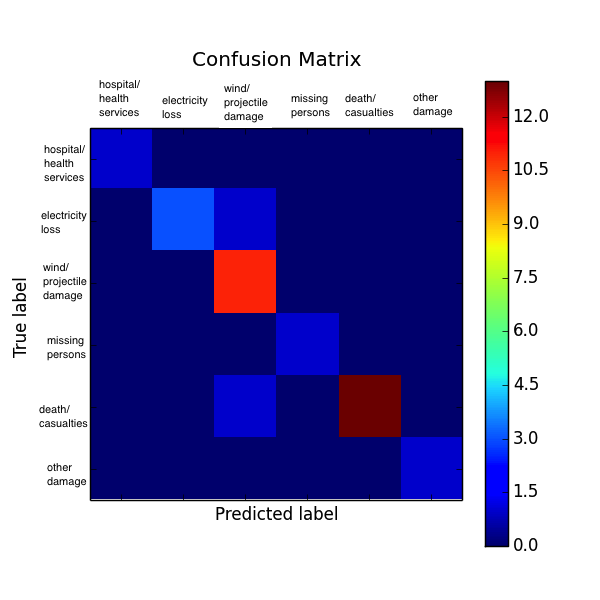
\includegraphics[width=90mm]{confusion_matrix}
\caption{Confusion Matrix of predicted labels using k-folds cross validation}
\label{cm}
\end{figure}


\begin{table}[t]
\centering
\begin{tabular}{|l|}
\hline
{\bf Correctly identified as damage or casualty}\\
\hline
xxxx\\
\hline
{\bf Incorrectly identified as damage or casualty}\\
\hline
xxxx\\
\hline
\end{tabular}
\end{table}

\section{Related Work}
\begin{itemize}
\item Extracting Information Nuggets from Disaster- Related Messages in Social Media
\item Practical Extraction of Disaster-Relevant Information from Social Media
\item Social Media Data Mining: A Social Network Analysis Of Tweets During The 2010-2011 Australian Floods
\item TweetTracker: An Analysis Tool for Humanitarian and Disaster Relief
\item Natural Language Processing to the Rescue?: Extracting “Situational Awareness” Tweets During Mass Emergency
\end{itemize}



\section{Conclusions and Future Work}
\begin{outline}
  \item Summarize what we did
  \item Mention limitations
  \item Summarize next steps
\end{outline}

\section{Acknowledgements}
This work was performed during the 2013 Eric \& Wendy Schmidt Data Science for
Social Good Fellowship at the University of Chicago, in partnership with the
Qatar Computational Research Institute. We are greatful to Gnip for providing
access to the historical tweets used in this analysis, as well as to all the
2013 DSSG Fellows who helped with data annotation.

\bibliographystyle{abbrv}
\bibliography{tweedr}

\end{document}




